%%%%%%%%%%%%%%%%%%%%%%%%%%%%%%%%%%%%%%%%%%%%%%%%%%%%%%%%%%%%%%%%%%%%%%%%%%%%%%%%
\pagebreak
\section{Introduction}

%%%%%%%%%%%%%%%%%%%%%%%%%%%%%%%%%%%%%%%%%%%%%%%%%%
\subsection{Motivation}
Automation has been instrumental to industrial manufacturing since the 1950s, replacing human workers from tasks
requiring high precision, speed and endurance. Notable breakthroughs in this period include the remotely controlled
mechanical manipulators called ``teleoperators'', developed at Argonne and Oak Ridge National Laboratories for handling
radioactive material, and the programmable Computer Numerically Controlled (CNC) machine tools. Built upon these
inventions, George Devol developed one of the earliest realization of industrial automation, replacing the human
operator of ``teleoperators'' with the CNC controller, creating the first robotic manipulators \cite{Murray1994}.

The end effector is the device at the end of the robotic manipulator, which directly interacts with the manipulated
object. Traditionally in industry the end effector is a simple gripper. Any object movement in this case requires
manipulating the whole arm, which is effective for transferring objects over large motion ranges but can be intractable
for tasks requiring precise movements. The recent vacuum based effectors face similar problems in object manipulation.
To handle finer motions, the common solutions in industry are either using custom designed end-effector or multi-finger
robot hands. The problem of robotic grasping typically refer to the use of gripper and multi-finger end effector to
manipulate objects. 70 years after the conception of the first robot arm, a general solution to finding a suitable grasp
for objects is still a challenging problem and an area of active research.

%%%%%%%%%%%%%%%%%%%%%%%%%%%%%%%%%%%%%%%%%%%%%%%%%%
\subsection{Use Case}
\picHereWidth{robocup_typical_objects}
{Typical objects in the Robocup@Home competition \cite{robocupRulebook2018}.}
{fig:robocup_objects}{0.9\textwidth}

This project focuses on the use cases of robotic grasping in the
\footnoteHref{http://www.robocupathome.org/}{Robocup @Home} league. The tasks in this competition are designed to
evaluate performance of autonomous robots in service robotic applications in a domestic environment. The objects to be
manipulated are ones that can be found in a typical household setting. Some examples of such objects can be seen in
figure \ref{fig:robocup_objects}. These objects can be placed on tables, shelves or in a dishwasher, whose locations
can be anywhere in an simulated apartment. Grasping tasks in such an environment is challenging than because of various
factors, including the variety of object shapes, the uncertainty of the robot manipulator and objects' locations,
and the many noise/disturbance sources which can interfere with the robot's perceptual sensors such as lighting
condition or object occlusion.

The platform used for the project's experiments is the robot chosen for the standard platform for the Robocup@Home
league, the
\footnoteHref{http://www.toyota-global.com/innovation/partner\_robot/robot/\#link02}{Toyota Human Support Robot (HSR)}
\cite{robocupRulebook2018}. The robot is equipped with a RGB-D sensor
(\footnoteHref{https://www.asus.com/3D-Sensor/Xtion\_PRO\_LIVE/}{Xtion PRO LIVE}), stereo camera and a wide angle camera
on the robot head, as well as a wide angle camera mounted on the two-finger gripper. The gripper also has a potentiometer
and a force sensor.

%%%%%%%%%%%%%%%%%%%%%%%%%%%%%%%%%%%%%%%%%%%%%%%%%%
\subsection{An overview of robotic grasping research}

\picHereWidth{bohg14-grasp_synthesis_mind_map}
             {Aspects which may influence generation of grasp hypotheses \cite{Bohg2014}.}
             {fig:grasp_synthesis_mind_map}{0.9\textwidth}
Synthesizing an optimal grasp from perceptual data is a challenging problem and is frequently addressed in
robotic research, resulting a myriad of approaches. Sahbani et al. \cite{Sahbani2012} classify grasp synthesis
into analytical and empirical approaches. Analytical methods consider mechanical properties of the contact
points between the gripper's fingers and an object \cite{Roa2015,Sahbani2012,Shimoga1996}, namely:
\begin{itemize}
\item Disturbance resistance: ability of the grasp to resist disturbances when the object is immobile, either by
form-closure (finger positions) or force-closure (forces applied by fingers).
\item Dexterity: ability of the robot hand to move the object to perform a specified task, or in any direction if
no task is specified.
\item Equilibrium: the combined forces and torques applied onto the object is null.
\item Stability: any displacement of an object caused by a disturbance will self-correct over time.
\end{itemize}
Instead of analyzing mechanical properties, empirical approaches rely on some form of grasp experience to synthesize
candidates. Sahbani et al. \cite{Sahbani2012} group empirical approaches based on whether they focus on observing humans
or objects. The first group of methods teach a robotic system to observe a human operator via different forms of
descriptors, then to reproduce the same grasp. These techniques are also known as learning by demonstration.
Methods focusing on object observation in general learn the association between object characteristics and gripper
configurations. The survey by Bohg et al. \cite{Bohg2014} argue instead to classify data-driven methods based on how
much information is assumed about the query object, specifically:
\begin{itemize}
    \item Approaches dealing with \emph{known objects} rely on a grasp experience database which contain suitable grasps
    for each encountered object. These approaches, therefore, focus on object recognition and pose estimation.
    \item Approaches for \emph{familiar objects} focus on finding a similarity metric and an object representation,
    from low (i.e. shape, color, texture) to high (i.e. category) levels, to match query objects with encountered
    objects.
    \item Approaches for \emph{unknown objects} identify local or global features from sensory data to for generating
    and evaluating grasp candidates.
\end{itemize}
The authors argue that this classification can better capture the diversity of empirical approaches as well as
the importance of perception in the process. In addition to the above classification, Bohg et al. \cite{Bohg2014}
also identify principal factors that may influence a grasp hypothesis, as shown in the mind map in figure
\ref{fig:grasp_synthesis_mind_map}.

Analytical approaches to synthesizing grasps generally rely on knowledge of the object, the gripper model and the
contact location of the fingers. These information is often inaccurate or unavailable in the real environment
because of noisy sensors as well as imprecise manipulator/gripper actuation. Indeed, analytical methods have been
shown to be unreliable in synthesizing stable grasps when applied on real robots
\cite{Kappler2015, Rubert2017, WeiszAllen2012}. Empirical approaches, however, as with other supervised machine
learning methods, demand labeled data. Generating a sufficiently large grasp experience knowledge base is often
time-consuming and expensive, while grasp simulation may not be close enough to the real world.

Data augmentation, the process of generating new samples by transforming real data, and data synthesis are popular
solutions to supplementing limited training data \cite{Fawzi2016, Shrivastava2017}, especially when applying deep
learning methods to solve image recognition and detection tasks. As grasp synthesis algorithms need 3D information
synthesizing the gripper configuration, RGB-D is often preferred over images as training data. The research in
\cite{Eitel2015,Gupta2014RGBDFeatures} proposes approaches to augmenting RGB-D data, whereas Mahler et al.
\cite{mahler2017} generates synthetic data to train a grasp quality predictor.

In order to leverage the successes of deep learning for various perception and grasping tasks, which are in general
supervised techniques, this project shall focus on data generation and augmentation for empirical approaches to grasp
synthesis using labeled data.

\todo{layout of the report}
%%%%%%%%%%%%%%%%%%%%%%%%%%%%%%%%%%%%%%%%%%%%%%%%%%%%%%%%%%%%%%%%%%%%%%%%%%%%%%%%
\pagebreak
\section{Related Work}
Empirical grasp synthesis techniques based on labeled data vary mainly in what type of perceptual data is taken into
consideration, how object-grasp representation is formulated based on such perceptual data, and how grasps are
evaluated. This section will review these aspects are handled in recent methods, as well as approaches to augment and
synthesize data relevant to grasping.

%%%%%%%%%%%%%%%%%%%%%%%%%%%%%%%%%%%%%%%%%%%%%%%%%%
\subsection{Extracting features from perceptual data for grasping}
Qi et al. \cite{Qi2016}, Porzi et al. \cite{Porzi2017} \todo{fill approaches}

As RGB-D cameras become more accessible and affordable, they are often chosen in robotic systems as the primary
perception sensor. While RGB-D data has been shown to provide richer features compared to pure 2D images for various
perception tasks \cite{lenz2015,Eitel2015,Gupta2014RGBDFeatures,jiang2011}, it is often unclear how to handle the
multi-modality of color and depth information.

Lenz et al. \cite{lenz2015} use deep auto-encoders to build a representation for each feature channel, reducing its data
dimensions. To handle the multi-modality of RGB and depth data, the authors also introduced a structured regularization
technique. Each modality (i.e. RGB and depth/surface normal) has a regularization term which will be added to each
hidden unit. In case of a $p-norm$, with $K$ hidden units, $R$ modalities, and N visible units, the regularization term
would be
\[f(W) = \sum\limits^K_{j=1} \sum\limits^R_{r=1} \left( \sum\limits^N_{i=1} S_{r,i} \lvert W^p_{i,j} \rvert \right)
^{1/p}, \]
where $S_{r,i}$ is $1$ if feature $i$ belongs to modality $r$ and $0$ otherwise.

Bo et al. \cite{Bo2013} build sparse coding dictionaries for RGB-D data using the K-SVD algorithm, and proposed to use
hierarchical matching pursuit (HMP) to compute a feature hierarchy for new RGB-D images. Each entry in the dictionaries
contain 8 channels calculated from RGB-D data: grayscale intensity, RGB, depth and surface normals in three axes.

\picHereWidth{Eitel_et_al-2015-depth_color_encodings}
{Different encodings of depth information \cite{Eitel2015}. From left: RGB, grayscale depth, surface
    normals \cite{Bo2013}, HHA \cite{Gupta2014RGBDFeatures}, and the color mapping of depth values proposed
    by Eitel et al. \cite{Eitel2015}.}
{fig:depth-encodings}{\linewidth}

In order to leverage the success of Convolutional Neural Networks (CNN) in capturing 2D features \cite{Gu2018}, several
multi-modal approaches convert depth data into three-channel images during the preprocessing step
\cite{Eitel2015,Gupta2014RGBDFeatures}. Gupta et al. \cite{Gupta2014RGBDFeatures} propose the HHA representation, which
encode the depth each pixel of the depth image with horizontal disparity, height above ground, and the angle between the
local surface normal and direction of gravity. Eitel et al. \cite{Eitel2015} propose to use convert the depth value
directly into RGB values using a jet color mapping. Examples of the different depth encodings can be seen in figure
\ref{fig:depth-encodings}. Two CNN models of the same architecture are then trained independently using depth and RGB
images to classify objects. Finally, features learned from the two models (the networks up until before the
classification layer) are concatenated as inputs to a fully connected layer which learns to combine them to recognize
objects. The paper showed that while surface normals proved to give better classification performance using depth
information alone, they require additional calculation on the input data and does not improve on results when combining
both RGB and depth images compared to the proposed color map encoding.

%%%%%%%%%%%%%%%%%%%%%%%%%%%%%%%%%%%%%%%%%%%%%%%%%%
\subsection{Object-Grasp representation}
Bohg et al. \cite{Bohg2014} parameterize grasps by (1) the \emph{grasping point} of the object where the gripper
should be aligned, (2) an \emph{approach vector} from which the gripper shall approach the \emph{grasping point},
(3) the \emph{wrist orientation} of the robotic hand, and (4) an \emph{initial gripper configuration}.
The article also categorized object-grasp representation approaches into ones which extract local (i.e. curvature,
contact area with the hand) or global features (center of mass, bounding box).

%%%%%%%%%%%%%%%%%%%%%%%%%%%%%%
\subsubsection*{Techniques based on global features}
As illustrated in figure \ref{fig:dexnet-data-gen}, Mahler et al. \cite{mahler2017} represent grasps in 2D images by
aligning the image center to the gripper central point and the image's middle row to the grasp axis. The grasp is
assumed to have an approach vector perpendicular to the table, and hence is characterized by the gripper center and the
angle of the gripper axis with respect to the table.
\picHereWidth{mahler_et_al-2017-dexnet_2-dataset_generation}
             {Dex-net 2.0 data generation pipeline \cite{mahler2017}.}
             {fig:dexnet-data-gen}{\textwidth}

Several methods use eigengrasps to represent the object-grasp relation in free space \cite{Goldfeder2011,Ciocarlie2009}.
Ciocarlie and Allen \cite{Ciocarlie2009} introduced eigengrasps and defined them as principal components of the dataset
of human hand configurations. Using this low-dimensional representation, the robot hand receive adjustments from a human
operator during grasp execution. The proposed Eigengrasp planner uses a simulated annealing algorithm to maximize a
quality metric $Q$ calculated from robot hand's posture and pose, where posture is represented using an eigengrasp.
Specifically,
\[ Q = \Sigma_i (1 - \delta_i) \]
for all desired contacts $i$, where
\[ \delta_i = \cfrac{|\mathbf{o_i}|}{\alpha}
              + \left(1 - \cfrac{\mathbf{\hat{n}_i} \cdot \mathbf{o_i}}{|\mathbf{o_i}|} \right), \]
in which the local surface normal $\mathbf{\hat{n}_i}$ and the distance between desired contact location and the
object $\mathbf{o_i}$ is related to the eigengrasp and hand position. $\alpha$ is a scaling factor make the first term
comparable to the second in the latter equation. Goldfeder and Allen \cite{Goldfeder2011} used the Eigengrasp planner
to generate the Columbia Grasp Database. Grasp planning is then done by matching the query object to one in the
database, then executing the best indexed grasp for the matched object.

\todo{need 1 more approach}

%%%%%%%%%%%%%%%%%%%%%%%%%%%%%%
\subsubsection*{Techniques based on local features} \label{subsub:object_grasp_local}

\picHereWidth{detry_et_al-2012-fig3-part_candidates}
{Generating part candidates with box-shaped region of interests \cite{Detry2012}.}
{fig:part_candidates}{0.7\textwidth}

Detry et al. \cite{Detry2012} attempt to apply grasp experience demonstrated on known objects to novel ones by finding
similar graspable regions. As illustrated in figure \ref{fig:part_candidates}, the part candidates are point clouds
extracted from applying a set of predefined region of interest (ROI) boxes on a known grasp from the database. Then a
the authors defined a distance metric for clustering similar candidate parts, and a dictionary of candidate parts is
created using only the central points of these clusters. Part candidates for new object are then matched against this
dictionary to find possible grasps for the familiar object part.

\todo{add illustration of rectangle method}
Several methods represent grasp candidates as rectangles positioned in RGB and/or depth images \cite{lenz2015,jiang2011},
corresponding with a bipedal gripper. The RGB-D image region within these rectangles is then used to score the
respective grasp using machine learning methods. These approaches are naturally limited in their ability to represent
the robot hand's approach vector, since rectangles in the images can only correspond with grasps roughly orthogonal with
the plane of the RGB-D camera \cite{Gualtieri2016}.

\picHereWidth{kappler_et_al-2015-fig8-local_shape_diff_viewpoints}
             {Local shape representations with different camera view points of the same grasp. Cyan lines represents the
              approach vectors while pink lines represent the camera viewpoint \cite{Kappler2015}.}
             {fig:local_shape_viewpoints}{0.8\textwidth}

Kappler et al. \cite{Kappler2015} extract local shape representations (or templates) of objects from point clouds
generated from object meshes at various camera view points. The templates are grids with predefined resolution
aligned with the plane tangent to the object surface at intersection point between grasp approach vector and the
object. Each point cloud will be projected onto the grid, where the grid cells with corresponding projected points
``contain the distance to that point as a value,'' and the other grid cells are considered either occlusion
(with height depends on the camera angle) or free space (with fixed height). Figure \ref{fig:local_shape_viewpoints}
illustrates how the local shape representations capture the different camera viewpoints.

Gualtieri et al \cite{Gualtieri2016} propose to represent a grasp candidate by the cuboid swept out by a two-fingered
gripper as it closes on the object, extracting the observed points from RGB-D clouds and sampling points unobserved by
all sensors within the region. In order to reduce dimensionality, the points in this cuboid region are then voxelized
into $60 \times 60 \times 60$ grid, then projected onto the three planes corresponding with the cuboid's principal axes.
For each projection, three images are generated: the average height maps of the occupied points ($60 \times 60$) and
unobserved region ($60 \times 60$), as well as the average surface normals ($60 \times 60 \times 3$), whose three
dimensions are interpreted as three channels in the image. These result in a total of 15 channels representing each
candidate grasp. In their experiments, this approach performs better than the above approach proposed by Kappler et al
\cite{Kappler2015}, but does not improve significantly over their previous approach, which used only three channels from
the surface normals for each projection. This approach did not consider RGB data, arguing that the improvement would be
insignificant considering the results from \cite{lenz2015}.

%%%%%%%%%%%%%%%%%%%%%%%%%%%%%%%%%%%%%%%%%%%%%%%%%%
\subsection{Grasp evaluation}

%%%%%%%%%%%%%%%%%%%%%%%%%%%%%%
\subsubsection*{Quick overview of classical grasp metrics}
\begin{table}[H]
    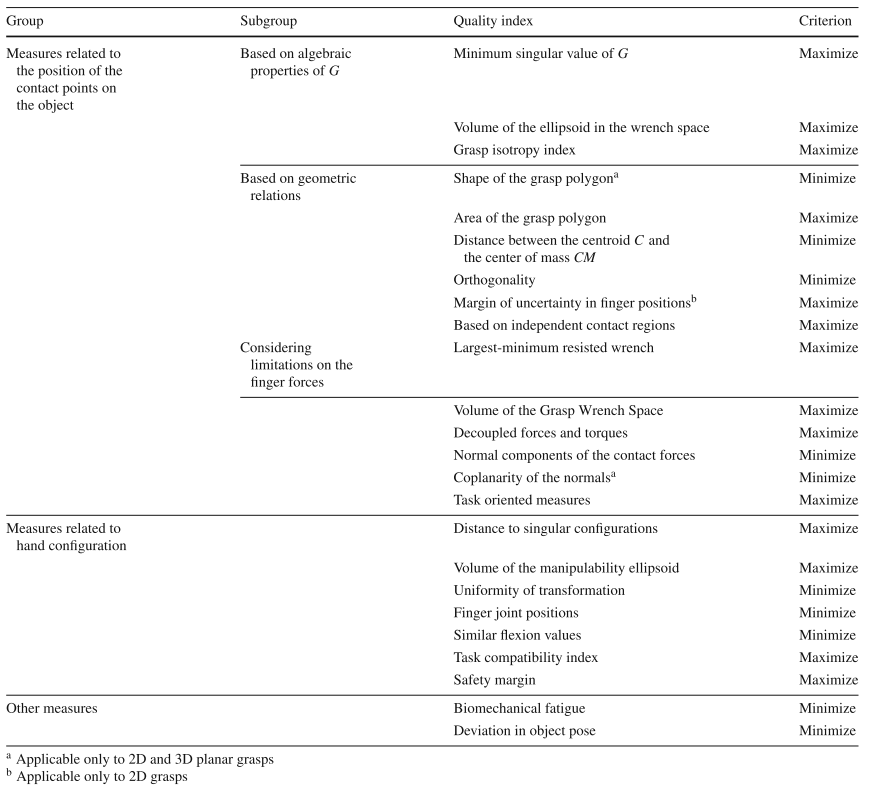
\includegraphics[width=\textwidth]{roa_suarez-2015-grasp_metrics}
    \caption{Grasp quality measures \cite{Roa2015}.}
    \label{table:grasp_metric}
\end{table}

Roa and Su{\'a}rez group grasp quality measures into approaches focusing on contact point position, hand configuration, and ones which combine both metric types \cite{Roa2015}.
\begin{itemize}
    \item Contact point grasp quality measures focus on the object's properties, friction constraints and form/force closure conditions.
    \item Hand configuration measures focus on studying the properties of the hand-object Jacobian $H$.
    \item Grasp measures can be combined serially or in parallel to capture different aspects of a grasp's quality. In the serial approach, one quality measure is applied to find several grasp candidates, then another metric is used to choose the optimal candidate. The parallel approach combines the different measures in a single global index.
\end{itemize}
Table \ref{table:grasp_metric} illustrates how contact point and hand configuration related approaches can be further categorized into subgroups, and include metrics based on bio-mechanical fatigue and deviation of object pose which are not encapsulated by the aforementioned groups.

Weisz and Allen \cite{WeiszAllen2012}
\todo{$\epsilon$-metric}

%%%%%%%%%%%%%%%%%%%%%%%%%%%%%%
\subsubsection*{Learning to predict grasp quality}
Learning rectangles \cite{mahler2017,jiang2011,lenz2015}
Kappler et al. \cite{Kappler2015}

\todo{to be filled}

%%%%%%%%%%%%%%%%%%%%%%%%%%%%%%%%%%%%%%%%%%%%%%%%%%
\subsection{Generating data for grasp success prediction}

%%%%%%%%%%%%%%%%%%%%%%%%%%%%%%
\subsubsection{Data synthesis for robot grasping}

The earlier approaches to grasp knowledge synthesis often generate geometrically sound grasps for known object models.
The agent then learns to match detected objects with these object models to find suitable grasps to execute. Notably
Goldfeder et al. \cite{Goldfeder2009CGDB} generate a database of form-closure grasps for 3D object models, in which each
grasp entry is represented by a pregrasp in the form of a two-dimensional eigengrasp \cite{Ciocarlie2009}, and the final
grasp pose. Grasps are sampled from a subspace of each robot hand's degree-of-freedom (DOF) space. The authors then used
a nearest neighbor algorithm to match each detected object to a model in this database \cite{Goldfeder2011} to find
grasp candidates.

Several grasp synthesis approaches generate perceptual data from object meshes at different viewpoints
\cite{mahler2017,Gualtieri2016,Kappler2015} for constructing a grasp knowledge database. Mahler et al. \cite{mahler2017}
use 3D mesh models from Dex-Net 1.0 \cite{mahler2016}, rescaling them to fit within the gripper's physical constraints.
Stable poses are computed for each object, and poses with probability of occurrence above a threshold are stored.
For each stable pose a set of grasps is sampled perpendicular to the table and collision-free. Rejection sampling
is used during grasp generation to ensure coverage of the object surface. Grasps are then ranked and selected using
a trained grasp quality metric. Finally, 2D images are generated from these grasp candidates as training data with the
antipodal axis aligned to the middle row of the image. Figure \ref{fig:dexnet-data-gen} provides a visualization of this
data generation process.

Kappler et al. \cite{Kappler2015} generate data using the \footnoteHref{http://openrave.org/}{OpenRAVE}
\cite{Diankov2010} simulator. Reference grasps are sampled using the geometric strategy available in OpenRAVE, where the
contact points are approach points, and the surface normals are approach vectors. For each approach point, 8 wrist
rotations around the approach vector and two translation offsets are applied, resulting in 16 candidate grasps per
reference grasp. Data points are then generated for each grasp using the local shape representation described in
subsection \ref{subsub:object_grasp_local}. A set of metrics is then applied to evaluate candidate grasps, creating the
data labels.

As robots can rarely acquire the comprehensive model of their environment from perceptual sensors, training data for
robot learning should reflect what is normally available to the robot's perception pipeline. As a result, this project
will focus on data synthesis approaches which generate grasp knowledge databases synthesizing and labeling perceptual
data.

%%%%%%%%%%%%%%%%%%%%%%%%%%%%%%
\subsubsection{Data augmentation}

For learned models to become robust to noise in real world sensors and to alleviate the scarcity of real data,
augmentation techniques are often applied to available data before training
\cite{Eitel2015,Kappler2015,Gupta2014RGBDFeatures}. As defined in \cite{Gu2018}, data augmentation refer to transforming
existing data ``without altering their natures.'' Which features exactly should be preserved during the augmentation
process depend on the data type.

With the relatively recent popularization of RGB-D sensors, few approaches exist to augment depth data. Eitel et al.
\cite{Eitel2015} sample noise patches of fixed size from real RGB-D data and divide them into five groups depending on
the number of missing depth reading in each patch. To create a final noise pattern, a pair of patches are sampled at
random from two different groups, then randomly added or subtracted with each other and optionally inverted. This
process is repeated until a specific number of patterns is generated. During training, at a predefined probability,
a noise pattern will be randomly selected from this set and applied to the depth sample to create the noised input.
Kappler at al \cite{Kappler2015} introduces noise to the object poses while sampling for reference grasps, before
generating each data point. Specifically, at the grasp approach point, the object is rotated around a random axis, then
a random offset is added to the surface pose. This variations of the object pose are intended to capture the errors in
calculating the surface normals and the surface noise during the reconstruction as described in subsection
\ref{subsub:object_grasp_local}. Gupta et al. \cite{Gupta2014RGBDFeatures} have a simpler approach, only adding a low
frequency white noise to the disparity images to augment the depth information.

In contrast many augmentation approaches have been developed for images. Several involves simple geometric
transformations such as mirroring, rotating, shifting \cite{Gu2018} or photometric such as color scaling, contrasting
\cite{Eigen2015}. Hauberg et al. \cite{Hauberg2016Diffeomorphism} propose an elegant method to learn these
transformations using diffeomorphisms. The authors first estimate the transformations for image pairs in each class.
These transformations are then used as observations to build a class-wise statistical model of transformations.
New transformations are then sampled from this model and applied to input images.
\todo{which of this can be applied to depth}

\todo{should adversarial approaches be included?}

%%%%%%%%%%%%%%%%%%%%%%%%%%%%%%%%%%%%%%%%%%%%%%%%%%
%\subsection{Task Compatibility}
%    In addition to stability, a successful grasping strategy also has to take into account the task to be performed with the grasped object. However, Sahbani et al. \cite{Sahbani2012} points out that incorporating task compatibility in to grasp synthesis, is still an open challenge because of the difficulty in modeling a task and the computational cost of finding a suitable grasp once a task is defined. These challenges are particularly relevant to analytic grasp synthesis, but is also not solved by empirical approaches. Methods which mimic human grasping alleviate the need for modeling tasks but is not fully automatic when facing new objects, while methods based on object observations have to generate many grasp candidates and face the same difficulty of task modeling as analytical approaches. One possible approach suggested by the article is to directly identify object features that are relevant to the requested tasks. Approaches to task modeling include methods based on manipulability ellipsoids \cite{Yoshikawa1990} and task space polytopes \cite{lee1997}, or building a task compatibility index measuring the similarity between the optimal directions of the manipulator and the movements required by a specific task \cite{chiu1988}.
